\section{Franciszek Data}
\label{sec:franek}

\textbf{Wzór Eulera:}
\[e^{ix} = cos x + isin x\]
\hspace{2cm}

\textbf{Zdjęcie capybary: Figure \ref{fig:capybara}} 

\begin{figure}[h]
    \centering
    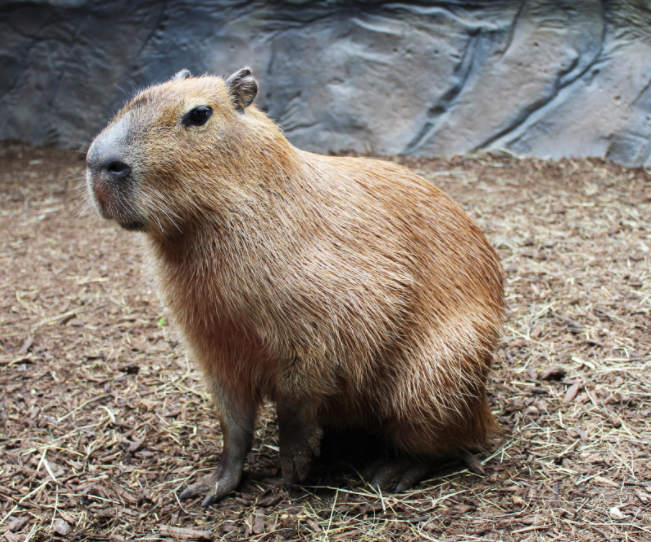
\includegraphics[width=0.6\textwidth]{pictures/Capy.jpg}
    \caption{Na zdjęciu widzimy Kapibarę}
    \label{fig:capybara}
\end{figure}
\hspace{2cm}

\textbf{Największe ssaki:}
\begin{enumerate}
    \item płetwal błękitny
    \item słoń afrykański
    \item nosorożec biały
\end{enumerate}
\hspace{2cm}

\textbf{Ryby polskie:}
\begin{itemize}
    \item Leszcz
    \item Ciernik
    \item Śledź
\end{itemize}
\hspace{2cm}
\newpage

\textbf{Macierz~\ref{tab:Jordan} to przykładowa macierz Jordana:}
\begin{table}[h]
\centering
\begin{tabular}{|c|c|c|} 
\hline
1 & 0 & 0 \\ \hline
0 & 2 & 1 \\ \hline
0 & 0 & 2 \\ \hline
\end{tabular}
\label{tab:Jordan}
\caption{Macierz Jordana}
\end{table}
\hspace{2cm}

\textit{\Large{Kapibara wielka}} - największy obecnie żyjący gatunek \underline{gryzonia} z rodziny kawiowatych. Jest to roślinożerne \textcolor{green}{zwierzęcie wodno-lądowe}, które zamieszkuje tereny \textbf{Ameryki Południowej.} \textit{Kapibara} wielka to \underline{gryzoń} o masywnej budowie ciała, gdyż jego masa może osiągać \textcolor{red}{nawet 65kg.}\\\par
\textit{\Large{Kapibary}} są zwierzętami \textbf{wodno-lądowymi} i prowadzą życie na otwartej przestrzeni. Poranki spędzają odpoczywając w \textcolor{blue}{wodzie}, zwłaszcza w zacienionym miejscu. Kapibary uwielbiają tarzać się w \textcolor{brown}{błocie.} Zwiększoną aktywność i żerowanie obserwuje się późnym \underline{popołudniem.} Kapibary jedzą powoli, więc żerowanie zajmuje wiele czasu.